\documentclass[]{spie}  %>>> use for US letter paper

\usepackage{graphicx}
\usepackage{subfigure}
\usepackage{amsmath}

\title{Supporting task-oriented collaboration in human-robot teams using semantic-based path planning}

\author{Daqing Yi and Michael A. Goodrich
\skiplinehalf
Brigham Young University, Provo, UT, USA 
}

\authorinfo{Further author information: (Send correspondence to Michael A. Goodrich)\\Daqing Yi: E-mail: daqing.yi@byu.edu\\  Michael A. Goodrich: E-mail: mike@cs.byu.edu}

\begin{document} 
\maketitle

\begin{abstract}
Improvements in robot autonomy are changing the human-robot interaction from low-level manipulation to high-level task-based collaboration.
For a task-oriented collaboration, a human assigns sub-tasks to robot team members.
%There usually exists difficulty for the human to define an accurate model for the robots, especially in the form of natural languages.
In this paper, we consider task-oriented collaboration of humans and robots in a cordon and search problem.
We focus on a path-planning framework with natural language input.
By the semantic elements in a shared mental model, a natural language command can be converted into optimization objectives.
We import multi-objective optimization to facilitate modeling the ``adverb'' elements in natural language commands.
Finally, human interactions are involved in the optimization search process in order to guarantee that the found solution correctly reflects the human's intent.
\end{abstract}

\keywords{Path planning, Multi-objective optimization, Semantic-based HRI}

\section{Introduction}

\begin{frame}{Modeling human intent}{Path Planning}
THe problem in modeling human intent
\begin{itemize}
\item incomparability in objectives
\item conflict in objectives
\item hardness in weighing the objectives
\item vagueness in importance selection
\end{itemize}
\begin{figure}
\centering
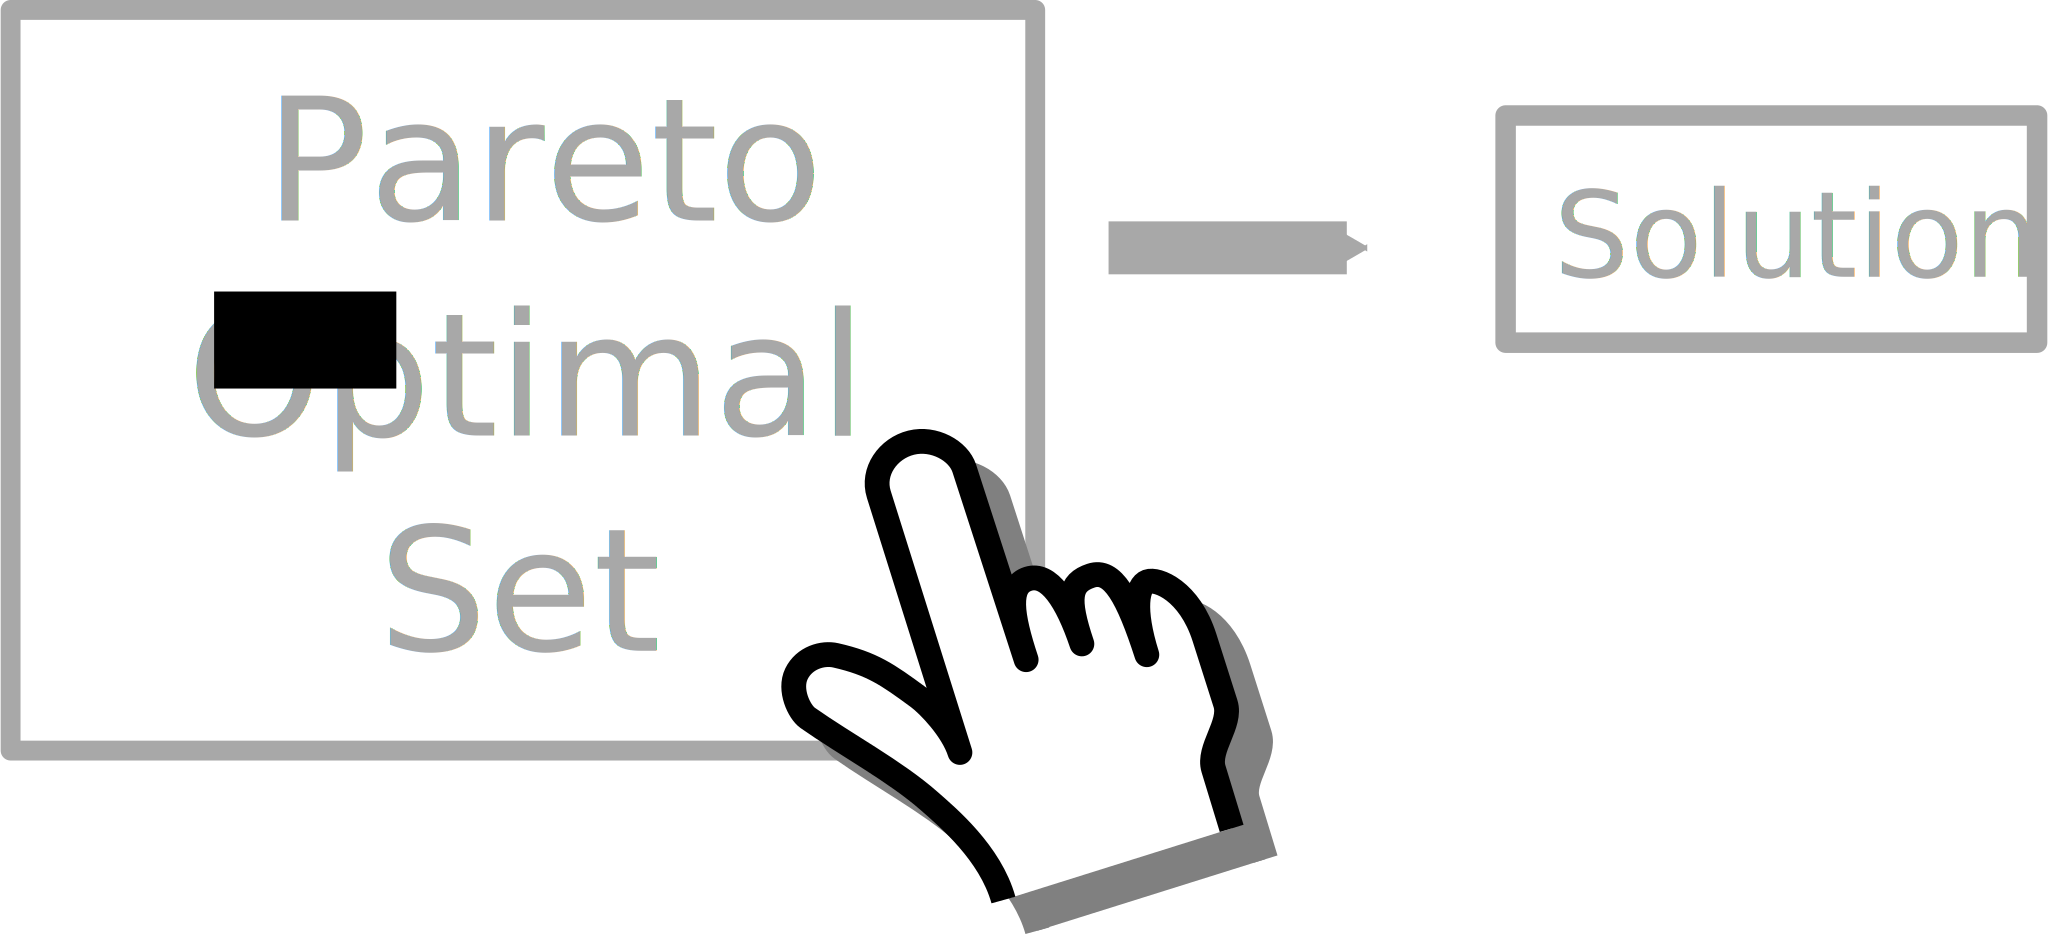
\includegraphics[width=0.6\linewidth]{figure/human_interactive_moo}
%\caption{}
\label{fig:human_interactive_moo}
\end{figure}
\end{frame}

\begin{frame}{Pareto Optimal}{}
\end{frame}

\section{Semantic labeling and command}
\label{sec:semantic}

%When human-robot teaming requires task-oriented collaboration in the real world, it is often necessary for the robot to translate a human's verbal command into a sequence and schedule of robot motions.

A shared mental model provides a common ground among the teammates of the collaborative process.
When the interaction between a human and a robot is based on natural language, the semantic objects must be shared by the team members so that the teammates can understand each other.
In a cordon and search task, the information depends greatly on the semantic labels of spatial objects.
It is natural to introduce a labeling process to generate the semantic objects on the map of the workspace.
These \emph{semantic labels} will be used in sub-task definitions and teammate interactions in the shared mental model.
We also need a \emph{task grammar} to define the sub-tasks and organize the semantic elements. 
Because terms and sentences usually imply different meanings in different types of sub-tasks, a task grammar could help the teammates understand the purposes of each other correctly.
In this way, a verbal command can be viewed as an action with logical constraints on a set of semantic elements. 
The form is determined by the task grammar. 

\begin{figure}
\centering
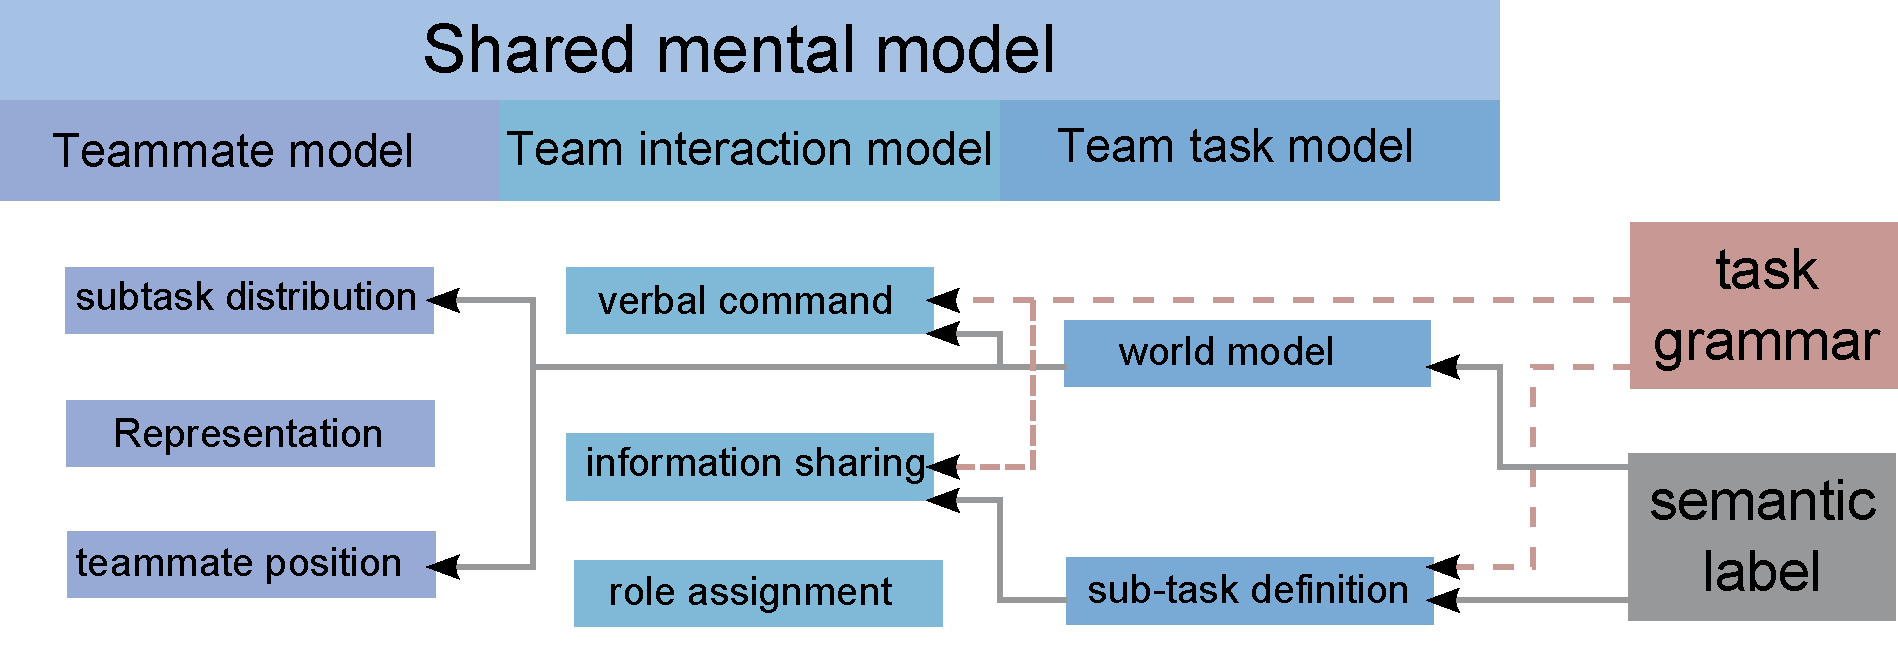
\includegraphics[width=0.7\linewidth]{./images/smm}
\caption{How task grammar and semantic labels support a shared mental model.}
\label{fig:smm}
\end{figure}

A shared mental model of a cordon and search team can be decomposed \cite{goodrich2013toward} into three sub-models.
We list only some elements that are relevant with a cordon and search task as following.
\begin{itemize}
\item
\textbf{A teammate model} provides the knowledge of teammates skills, abilities and tendencies.
\begin{itemize}
\item A \emph{sub-task distribution} indicates how the sub-tasks are assigned to team members.
\item The \emph{teammate positions} indicate the positions of the teammate, localized relative to the spatial semantic objects.
\item The \emph{representation} indicates how the teammate encodes information and problems.
\end{itemize}
\item 
\textbf{A team interaction model} provides the knowledge of roles, responsibilities, information sources, communication channels and role interdependencies.
\begin{itemize}
\item A \emph{role assignment} defines the roles of the members in a team.
\item A \emph{verbal command} describes the format of a command.
\item An \emph{information sharing} represents the information exchange format between team members.
\end{itemize}  
\textbf{A team task model} provides the knowledge of procedures, equipment, situations, constraints.
\begin{itemize}
\item A \emph{semantic world model} is a representation of the workspace with semantic labels.
\item A \emph{sub-task definition} defines the sub-tasks and its objectives.
\end{itemize}
\end{itemize}

Figure \ref{fig:smm} illustrates how these elements in a shared mental model depend on the task grammar and the semantic labels.
The task grammar and semantic labels support the world model and the sub-task definitions.
The world model and the sub-task definitions can then be used to generate verbal commands and help information sharing.
%Also the semantics in the world model can also help to describe how the sub-tasks are distributed to team members and the positions of the teammates in task execution.

Consider the cordon and search for a human-robot team in an urban area.
The labeling process is run before the cordon and search starts. 
Semantic labels are assigned to the sub-regions and the objects in the map.
Supplementary information can be attached to expand the support to different tasks.
We also expect that semantic labels are used to support a more flexible grammar.
We categorize the labels into three types.
\begin{itemize} 
\item \textbf{Indoor} 
The ``indoor'' label defines the region of an indoor environment in the search space.
\item \textbf{Outdoor} 
The ``outdoor'' label defines the region of an outdoor environment in the search space.
There are several sub-types on an outdoor label.
For the purpose of this paper, we consider only three.
\begin{itemize} 
\item \emph{market}: 
The ``market'' label usually defines sources of information, where there is high probability of interested events occurring.
\item \emph{risky}: 
The ``risky'' label indicates potential risks by prior knowledge. 
This implies that these regions have potential risks, which will be considered when safety is an objective in path planning.
\item \emph{unknown}: 
We usually consider unlabeled regions as ``unknown'' by default, which indicates the lack of prior information.
Thus, there is nothing special to be noticed in these regions.
\end{itemize}
\item \textbf{Feature} 
The ``feature'' label defines the objects in the search space.
They can be used for objects of interest, location indicators and etc.
%This will be used for 
There are two types of feature labels, which are
\begin{itemize} 
\item \emph{2D}: ``2D'' label defines the objects on the ground.
\item \emph{2.5D}: ``2.5D'' label defines the objects on the walls of the architectures.
\end{itemize}
\end{itemize}

Figure \ref{fig:Label} illustrates possible semantic labels for a notional world.

\begin{figure}[tbph]
\centering
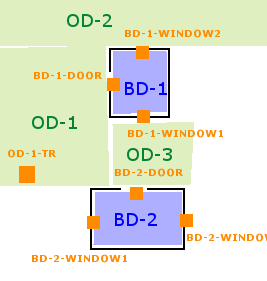
\includegraphics[width=0.4\linewidth]{./images/newLabel-text}
\caption{A labeled map of an urban environment.}
\label{fig:Label}
\end{figure}

Given the semantic labels of a spatial world model, we can define a task grammar by the characteristics of the sub-tasks.
We assume a task grammar that specifies a task, one or more constraints, and one or more adverbs that specify how the task should be performed or how the constraints should be managed.
Equation \ref{eq:task_grammar} is an example of a task grammar that is used in a cordon and search task.
\begin{equation}
\label{eq:task_grammar}
\begin{aligned}
< Start > \rightarrow & < CommandPhrase > \\
< CommandPhrase > \rightarrow & < ScreenCommand > \mid < ProceedCommand > \\
< ScreenCommand > \rightarrow & < Adverb > \mbox{ Screen the } < FeatureQuantifier > < Feature > \mbox{ of the } \\
& < BlockId > \\
< ProceedCommand > \rightarrow & \mbox{ Proceed } < Adverb > < PrepPhrase > \mbox{ to the } < FeatureQuantifier > \\ 
& < Feature >  \mbox{ of the } < BlockId > \\
< Adverb > \rightarrow & \mbox{ covertly } \mid \mbox{ safely } \mid \mbox{ quickly } \mid \mbox{carefully}\\
<FeatureQuantifier> \rightarrow & \mbox{ back }  \mid \mbox { front } \mid \mbox{ side } \\
<Feature> \rightarrow & \mbox{ door } \mid \mbox{ window } \mid \mbox{ exits } \\
<BlockType> \rightarrow & \mbox{ BD- } \mid \mbox{ OB- } \\
<PrepPhrase> \rightarrow & < PrepSegment > \mbox{ the } < BlockId > \mid \mbox{ between the } < BlockId > \\
& \mbox{ and the } < BlockId > \\
< BlockId > \rightarrow & < BlockType > < Id > \\
<PrepSegment> \rightarrow & \mbox{ around } \mid \mbox{ left-of } \mid \mbox{ right-of }
\end{aligned}
\end{equation}

For example, if a human tells a robot to ``carefully screen the OB-2'', this command defines a sub-task as a ``screen'' action.
``OB-2'' is a semantic label, which constrains the task to specific work region.
Besides what to do in a sub-task, this verbal command also implies how to evaluate the performance of this sub-task.
Some of the objectives inherit from the properties of a screen action,
the other objectives are from the adverb, e.g. ``carefully''.
This turns the path-planning problem in the sub-task into a multi-objective optimization problem as described in the next section.


\section{Interactive multi-objective optimization}
\label{sec:moo}

The adverb in a sentence can be very important and informative.
In a cordon and search task, using ``carefully'', ``quickly'' or ``covertly'' imply very different ways of performing the task. 
More generally, a verbal command from a human contains multiple objectives and constraints, which means that the robot's path-planning problem is a multi-objective optimization problem.
Table \ref{tab:adverbs} gives an example on different objectives implied by different adverbs in cordon and search. 
Four adverbs indicate different objectives that the robot's path planner may need to respect.

\begin{table}[h]
\caption{Different objectives implied by different adverbs.} 
\label{tab:adverbs}
\begin{center}  
\begin{tabular}{|c|c|c|c|c|}
\hline  
\rule[-1ex]{0pt}{3.5ex} Adverb & Covertly & Safely & Quickly & Carefully \\ 
\hline
\rule[-1ex]{0pt}{3.5ex} Objectives & 
\parbox{.18\linewidth}{
\begin{description}
\item $ \min $ visibility
\item $ \max $ smoothness
\end{description}  
} & 
\parbox{.18\linewidth}{
\begin{description}
\item $ \min $ exposure
\item $ \min $ danger
\end{description}  
}  & 
\parbox{.18\linewidth}{
\begin{description}
\item $ \min $ path length
\end{description}  
}  & 
\parbox{.18\linewidth}{
\begin{description}
\item $ \max $ smoothness
\item $ \min $ collision risk
\end{description}  
}   \\ 
\hline 
\end{tabular} 
\end{center}
\end{table} 

%Multiple objectives inherently exist in both layers of planning because adverbial modifiers from the human do not ``cleanly'' map to unique metric-based performance objectives.

Notice, as illustrated in Table \ref{tab:adverbs}, that the robot requires a precise definition so that the problem is mathematically solvable.
By contrast, a human may convey and process the information in fuzzier terms.
In terms of the representation element of the teammate model, this means that there is a mismatch between the human and the robot.
More specifically, there is a mismatch between the precise mathematical objectives required by the robot and the possibly ambiguous adverbial modifier specified by the human.
To solve such a problem, we propose a posterior method that allows the robot to specify a range of possible solutions, and allows the human to select from this range.

Specifically, we use the notion of \emph{Pareto optimality} to evaluate the solutions in a multi-objective optimization problem.
A solution is called ``Pareto optimal'' if no other solution has better fitness values in all the objectives.
This means that a Pareto optimal solution cannot be improved on one objective without downgrading other objectives.
A set that consists of all the Pareto optimal solutions is a \emph{Pareto front}.
Figure \ref{fig:moo} illustrates a Pareto front for a minimization problem.

\begin{figure}
\centering
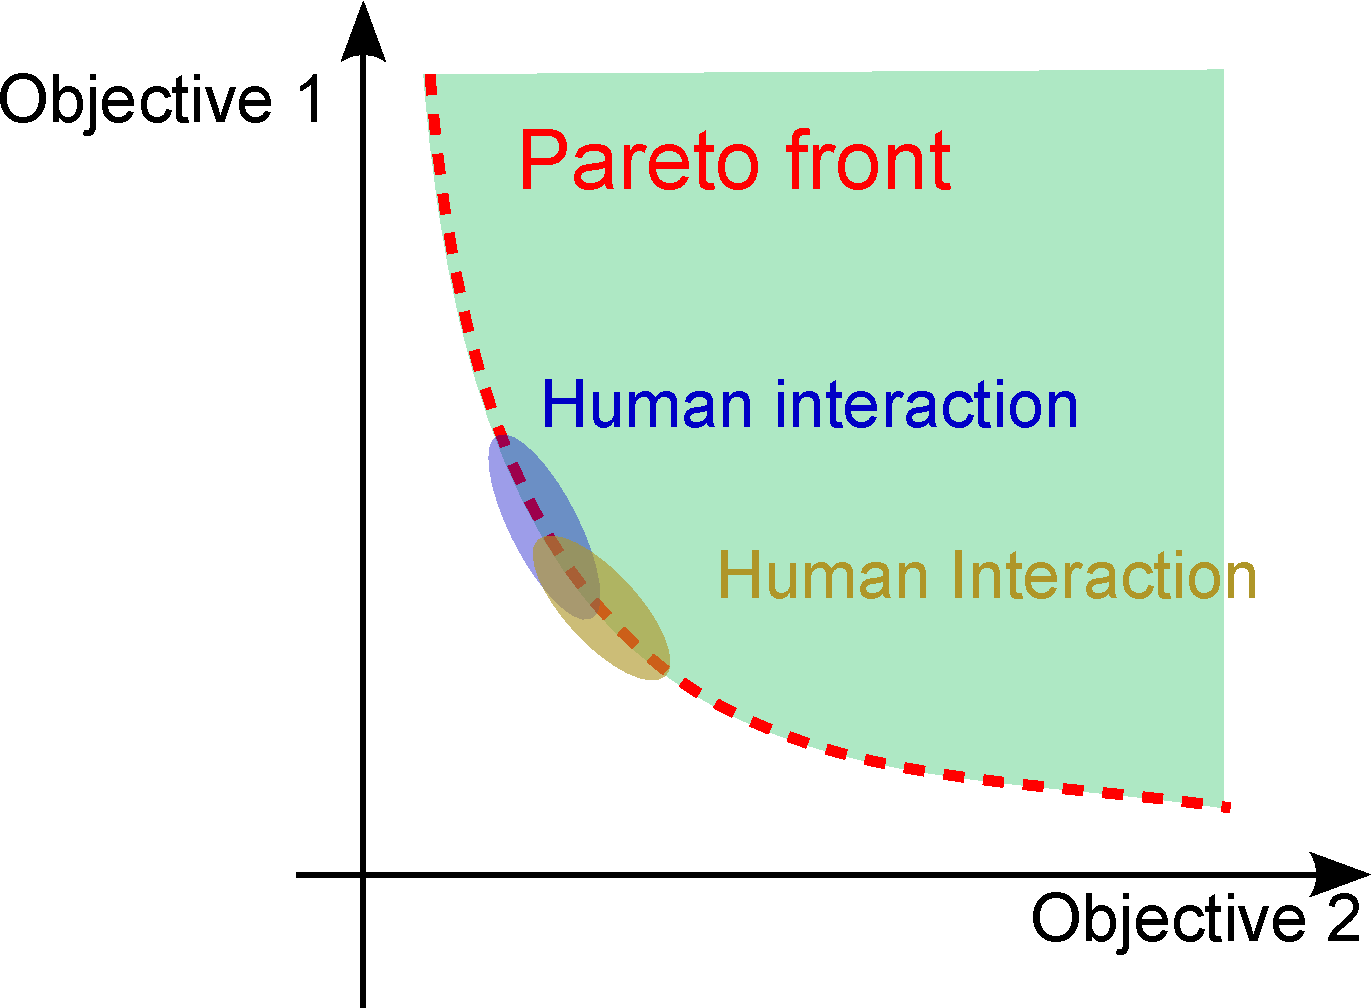
\includegraphics[width=0.4\linewidth]{./images/moo}
\caption{Interactive multi-objective optimization.}
\label{fig:moo}
\end{figure}

The task grammar from Section \ref{sec:semantic} allows two different types of information to be shared among the human supervisor and the robot:
the specific task to be performed (encoded as the verb and noun) and an adverbial qualifier on how the task should be performed.
The verb and noun specify hard constraints that must be satisfied by the solution generated by the robot's path planner.
By contrast, the adverbial modifier represents a soft constraint that the path should satisfy.

We assume that the soft constraint is fuzzy, meaning that there are several possible paths that would satisfy the soft constraint, and selecting from among these possible paths. requires an ability to balance various tradeoffs.
The Pareto front represents all possible tradeoffs, so a specific adverbial modifier does not specify a single point in the Pareto front, but rather a region of the Pareto front; any solution within this region might match the human's intent.
This is illustrated on Figure \ref{fig:moo} as  the shaded ovals.
We are developing a tool that allows a human to interactively explore this region to select a path that balances tradeoffs which satisfy human intent.
This tool bridges the difference between the way a human and a robot represent a task, and thus facilitates more effective shared mental models.
 
%With a Pareto front obtained, a human interactive decision process can be used as a posteriori method \cite{5585740}.
%The interaction process iteratively imports a human's selection in search for the most preferred solution.
%The human's selection could provide either a sub-region in the given optimal set or an improvement on the objective definition.
%It is expected that the solution set gradually converge to the most preferred one.

In terms of the robot's path planner, since the solutions generated from the multi-objective planner are Pareto optimal, information communicated from the planners to the human allow the human to refine their intent by selecting among these tradeoffs.
We introduce this interactive multi-objective optimization to solve the path planning problem modeled from a human verbal command.

Unfortunately, the solution space of a path planning problem has been greatly expanded.
This increases the difficulty of solving the multi-objective optimization problem.
Following related work on blending metric-based and topological approaches to path planning, we are developing a robot path representation using waypoints and trajectories that connect two neighboring waypoints.
This enables a two layer planning in order to enhance the planning efficiency:
\begin{itemize}
\item A coarse layer generates the waypoints.
\item A fine layer generates the trajectories between the waypoints.
\end{itemize}
The planning in both layers follow the same objectives and constraints.

When we have a shared mental model with semantic labels and a path planner that solves the multi-objective optimization problem, we can provide an efficient framework of optimized path-planners that can be flexible and adaptive to new forms of objective definitions from new scenarios and new information sources.


\section{System}
\label{sec:system}

In this paper we use the formulas from Kennedy's most recent definition of PSO~\cite{4223164}.
It can be easily extended to many versions of PSO.
This version of PSO includes a constricted position update rule, a personal best update and a star topology formed by a global best update.
The constricted position update rule is
\begin{subequations}
\label{eq:pso_alg}
\begin{equation}
\label{eq:up_vel}
\begin{aligned}
v_{ij}(k+1) = &  \chi [ v_{ij}(k) 
 + \phi^{P} u^{P}_{ij}(k) (x^{P}_{ij}(k) - x_{ij}(k))\\
 & + \phi^{G} u^{G}_{ij}(k) ( x^{G}_{ij}(k) - x_{ij}(k)) ],
\end{aligned}
\end{equation}
\begin{equation}
\label{eq:up_pos}
x_{ij}(k+1) = x_{ij}(k) + v_{ij}(k+1).
\end{equation}
\end{subequations}
$ x_{ij}(k) $ represents the position of particle $ i $ in dimension $ j $ at time $ k $.
$ v_{ij}(k) $ similarly represents the velocity of particle $ i $ in dimension $ j $ also at time $ k $.
$ x^{G}_{ij}(k) $ and $ x^{P}_{ij}(k) $ are global (actually topology) and personal best positions observed by the swarm and the particle respectively. 
$ u^{G}_{ij}(k) $ and $ u^{P}_{ij}(k) $ are independent random values drawn from $ [0,1] $.
$ \chi \in ( 0, 1 ) $, $ \phi^{P} $ and $ \phi^{G} $ are algorithm parameters.
The personal best update is
\begin{equation}
\label{eq:pb_up}
x_{i}^{P}(k) = \arg \max_{ x \in \{ x_{i}(k), x_{i}^{P}(k-1) \} } f(x).
\end{equation}
The global best update is
\begin{equation}
\label{eq:gb_up}
x_{i}^{G}(k) = \arg \max_{ x \in \{ x_{i}(k), x_{i}^{G}(k-1) \} } f(x).
\end{equation}
The share of the global best leads to a star topology in the swarm.

When particle $ i $ finds a position that is better than the current global best, it updates the global best and its personal best.
The swarm moves to a new global-best stagnation.
In this case, there is $ x_{i}(k) = x_{i}^{P}(k) = x_{i}^{G}(k) $ in the particle.
Equation \eqref{eq:up_vel} becomes
\begin{equation}
v_{ij}(k+1) = \chi [ v_{ij}(k) 
 +( \phi^{P} u^{P}_{ij}(k) + \phi^{G} u^{G}_{ij}(k) ) (x^{G}_{ij}(k) - x_{ij}(k))  ].
\end{equation}
As the inertia of the previous velocity $ v_{ij}(k) $ will decay to zero,
the particle is attracted to $ x^{G}_{ij}(k) $ as $ \phi^{P} u^{P}_{ij}(k) + \phi^{G} u^{G}_{ij}(k) \geq 0 $.
This particle can be viewed as a leader of this swarm.
The topology is given in Figure \ref{fig:leader_follower}.
\begin{figure}[tbph]
\centering
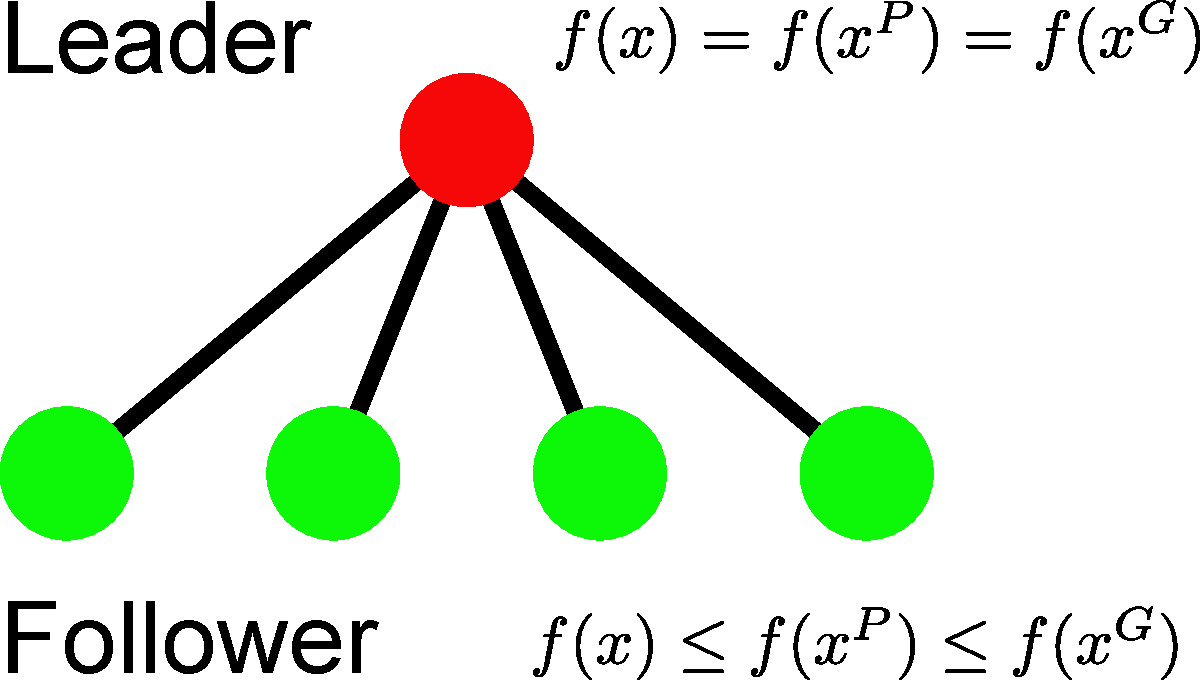
\includegraphics[width=0.5\linewidth]{./fig/leader_follower}
\caption{A leader-follower relationship.}
\label{fig:leader_follower}
\end{figure}

The star topology supports the leader competition among the particles.
The particle that finds a new global best becomes the leader of the swarm.
The other particles are the followers, which are attracted to the leader by the impact of the global best.
By Property \ref{prop:unconverge_neq_gb}, we know that a particle will never stop moving if the personal best and the global best are inconsistent.
Thus, we can view the movements of the followers are sampling in the solution space to solve the inconsistency between its own personal best and the global best.
The input to each particle from the topology of the swarm is only the global best.

\subsection{A feedback cascade model in a particle}

With the global best as the input, we model the behavior of a particle as a \emph{feedback cascade system}.
As shown in Figure \ref{fig:sys_flow}, this system is comprised of two components that form a feedback system structure.
These two components are 
the \emph{input-update component} for the personal best ($ x^{P}_{i}(k) $) and the global best ($ x^{G}_{i}(k) $), 
and the \emph{position-update component} for particle position ($ x_{i}(k+1) $), which depends on the inputs $ x^{G}_{i}(k) $ and $ x^{P}_{i}(k) $ as well as the last position $ x_{i}(k) $.

\begin{figure}
\centering
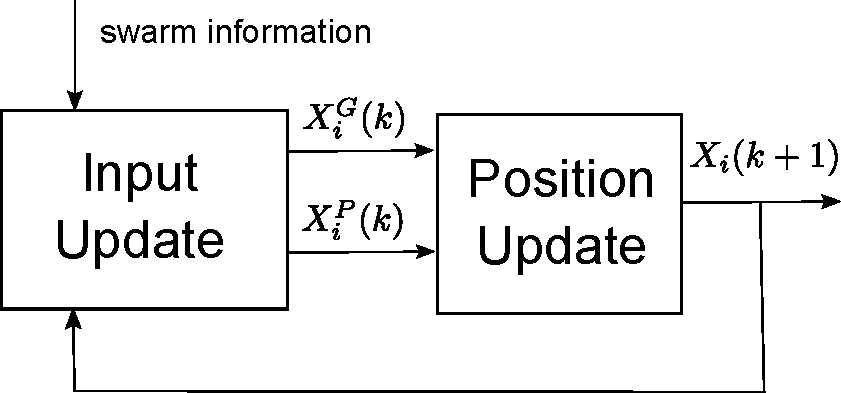
\includegraphics[width=0.85\linewidth]{./fig/sys_flow.pdf}
\caption{System structure of Particle.}
\label{fig:sys_flow}
\end{figure}

\begin{figure}
\centering
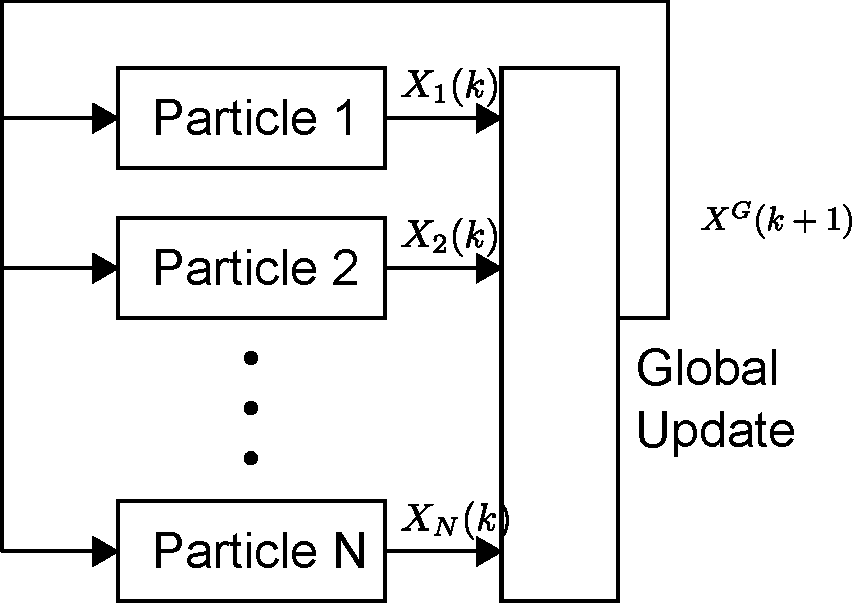
\includegraphics[width=0.6\linewidth]{./fig/pso_sys_flow.pdf}
\caption{System structure of Swarm}
\label{fig:pso_sys_flow}
\end{figure}

In the position-update component, the position at each dimension is updated by using the values from the $ x^{G}_{i}(k) $ and the $ x^{P}_{i}(k) $ in the corresponding dimension.
By Equation \eqref{eq:pso_alg}, we can decompose the position-update component into subcomponent in each dimension.
As shown in Figure \ref{fig:sys_flow}, the subcomponents in the position-update component form a parallel connection.
From \eqref{eq:pso_alg}, we can write a linear form of the position update component in one dimension.
\begin{equation}
\label{eq:pso_up_linalg_simp}
X(k+1) = A(k) X(k) + B(k) U(k)
\end{equation}
with
$ A(k) = \begin{bmatrix}
\chi & - \chi \phi^{G} u^{G}(k) - \chi \phi^{P} u^{P}(k)
\\ 
\chi & 1 - \chi \phi^{G} u^{G}(k) - \chi \phi^{P} u^{P}(k)
\end{bmatrix} $
and
$ B(k) = \begin{bmatrix}
\chi \phi^{G} u^{G}(k) & \chi \phi^{P} u^{P}(k)
\\ 
\chi \phi^{G} u^{G}(k) & \chi \phi^{P} u^{P}(k)
\end{bmatrix} $.
The system state is $ X(k) = [ v(k), x(k) - x^{*} ]^{T} $, and the system input is $ U(k) = [ x^{G}(k) - x^{*} , x^{P}(k) - x^{*} ]^{T} $.
\footnote{$ x^{*} $ means a reference point to the system.
When applying to the PSO, it can be a local optimum, a global optimum, or an estimated optimum.
We use it as a reference point to check the bounds.}
With a new $ x(k+1) $, the personal best update component will update the personal best $ x^{P}(k+1) $ that are fed into the position update component.

The input-update component consists of a \emph{global-best input} and a \emph{personal-best update}.
The personal best and global best are fed into the position-update component as input.
As in Figure \ref{fig:sys_flow}, the global-best input only takes the input from the swarm.
Thus the state to the reference point $ x^{R} $ is $  x^{G}(k) - x^{*} $.
The personal-best update compares the current $ x(k) $ with the $ x^{P}(k-1) $.
If  $ x_{i}(k) $ is better, the personal best is updated with it.
We can write the personal-best update as 
\begin{equation}
\label{eq:pso_input_up}
U = g^{PU}(V)
\end{equation}
with $ U = x^{P}(k) - x^{*} $ 
and $ V = x(k) - x^{R} $
from \eqref{eq:pb_up}. 

In Figure \ref{fig:sys_flow}, the position of a particle is modeled into a system with the input $ x^{G}(k) $ and the output $ x(k) $.
By using this model, we can have the system structure of a swarm in Figure \ref{fig:pso_sys_flow}.
There is a \emph{global update} that reads the states of all the particles and determine whether the global best should be updated.
The global best is fed back to all the particles for the next optimization iteration.



\section{Summary}
\label{sec:summary}

In this paper, we use a human path to form a path constraint and seek to maximize the information gathered by a robot gathered in a search task.
The resulting information maximization path planning is identified as a constrained submodular orienteering problem on a multi-partite graph.
We present an anytime algorithm that used a planning heuristic based on backtracking to efficiently find a high quality path.
We use a node freeze process to avoid an exhaustive search, yet we prove that this process always preserves the ability of the algorithm to find an optimal solution.
We have also shown empirically that this approach substantially reduces the complexity of the resulting search.

\acknowledgments     %>>>> equivalent to \section*{ACKNOWLEDGMENTS}       
We would like to thank the Robotics Collaborative Technology Alliance for providing funding for this work.
The views of this paper do not necessarily reflect the views of the funding agency.

\bibliography{reference}   %>>>> bibliography data in report.bib
\bibliographystyle{spiebib}   %>>>> makes bibtex use spiebib.bst

\end{document} 